\chapter{Introduction} % Main chapter title


\label{Chapter1} % For referencing the chapter elsewhere, use \ref{Chapter1} 

\lhead{Chapter 1. \emph{Introduction}}
% \HRule \\[0cm]
Since recent years, web applications are becoming a popular alternative to traditional desktop applications. To access a web application, the end-user is only required to maintain a functioning web-browser, whereas the application vendor can deploy and update the application independent of end-users’ system configurations. During the evolution of a web application, it is repeatedly modified to add new functionality, fix bugs or adapt the GUI (Graphical User Interface) to improve the user experience. After such modifications, it is not uncommon to encounter unintended side-effects in the application in the form of new bugs or re-emergence of old bugs. Such side effects usually occur as a result of changing system or component configurations, improper version control, applying incorrect or incomplete bug fixes etc. and can negatively affect the quality of the existing functionality. 

To ensure that after such modifications the application maintains its quality and still fulfills the existing specifications, regression tests are performed on the application under test (henceforth referred as AUT). Software developers typically run the existing test-suite along with a set of test inputs and oracles — a mechanism to assess the test output, on a newly developed version to make sure that the code and functionality carried over from older version behaves as expected.

Depending upon the development cycle, project size and available resources, regression tests can be performed at different abstraction levels, commonly as unit, integration and system testing. Unit tests are intended to test small pieces or modules of code, such as functions and classes, whereas integration tests are aimed to test the system as composition of different components. System level tests are performed at higher abstraction level similar to integration tests, however their goal is to check whether the software meets the requirements specifications. 

Intuitively, in case of web applications the system testing can be done at the GUI level, since majority of web applications’ functionality is accessed through this layer. In traditional sense, regression testing at GUI level abstracts away finer grained internal details by treating the AUT as a black-box. Such testing helps developers to identify the undesired  changes or an absence thereof in required functionality of the application, since the GUI might have changed significantly while the underlying application has not. However, as the application size increases, GUI testing becomes more complicated as a typical GUI test involves multiple sequential operations since certain functionalities are only accessible through a series of GUI events. For example, to purchase an item in a typical e-commerce web application a user would need to perform sequential events such as login, add product to cart, fill payment details and finally checkout. This flow can vary depending on additional functionality such as purchasing pre-selected products, favourites etc. As possible number of paths and sequences increase, generating test inputs and applying test oracles becomes more difficult and costly. Additionally, different browsers implement different technologies which might result in varied rendering of the GUI, making regression testing more complicated.

To reduce the costs incurred with manual testing, many developers choose to automate regression tests using frameworks such as Selenium \cite{websiteSelenium}. The Selenium project provides the \textit{Webdriver API}, to test dynamic web 2.0 applications. The API ‘drives’ i.e. controls the web browser in a manner that it emulates all possible user interactions with the application, such as clicks, form-inputs, file uploads etc. Compared to manual tests, such automated tests can be combined with Continuous Integration tools in order to be run more often, typically after new code is pushed to the version control repository. 

When a web application evolves from some previously tested and released version V0 to a newer version V1, existing Selenium test suite is executed on V1. Ideally, if one or more tests executed successfully on V0 fail to achieve the same result on V1, the new changes have possibly introduced regression faults in the AUT and these test cases can be used to further investigate and fix the regression faults. In reality, this approach not always effective as it relies heavily on the quality and robustness of the existing test suite. 

As the web application continues to evolve, the robustness of Selenium tests decreases over time. For newer versions, given pre-written tests do not achieve the same functional coverage as they do for the version the tests are originally written for. Considering the aforementioned example of two subsequent versions V0 and V1 of the AUT, if the outcome of regression changes results in version V1 missing an ‘add-to-cart’ button which the initial version V0 had; it is not possible to reach subsequent functionalities of V1, such as ‘order-confirmation’ or ‘payment’. In this scenario, the test corresponding to ‘add-to-cart’ functionality is broken and the desired functional coverage is not reached unless the test is fixed. This issue is also known as Reachability problem.

Intuitively, robustness of Selenium tests can be defined in terms of their stability and effectiveness to achieve the same functional coverage across different versions of the AUT. The reasons for decreasing robustness and failures of Selenium tests can include changed or reordered functionality, modified GUI element locators and changed structural markup, random page loading times and timeouts, unfinished JavaScript and Ajax calls etc. Such non-robust tests exhibiting decreased functional coverage can be unsuitable for regression testing unless these tests are modified. In other words, if the Selenium tests are not robust enough, the regression testing is likely to be ineffective. In order to modify such tests, developers need to invest time and efforts to analyze the undesired functionality changes, identify test failures manually and maintain such test-suites. 

Considering the current state-of-the-art technologies to the extent of my knowledge, thus far there has been no research in the area of assessing the stability of Selenium tests across different versions of the web application. Currently there is no such technique to determine the robustness of Selenium tests over the version history of web applications to help developers write more robust tests and to understand the reasons behind brittleness of Selenium regression tests. 
\begin{figure}
% [htbp]
	\centering	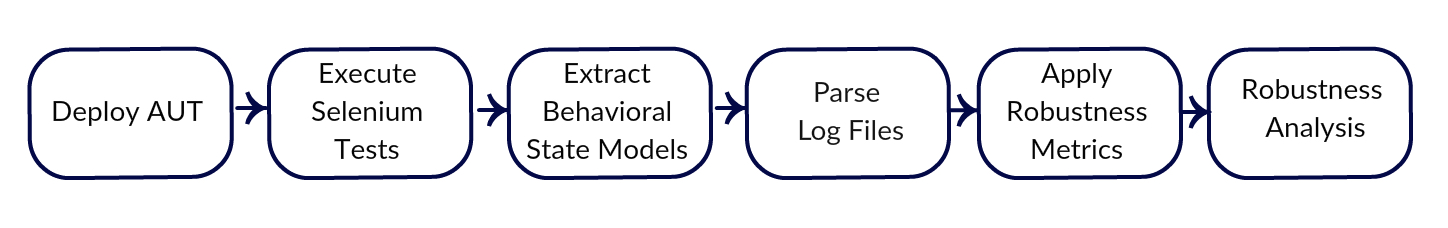
\includegraphics[width=\textwidth]{./Figures/thesisoverviewsmall.jpg}
%     [width=5cm, height=3cm]
% 		\rule{35em}{0.5pt}
	\caption{Setup required for the robustness analysis}
	\label{fig:thesisoverview}
\end{figure} 
The primary goal and scope of this thesis is to measure the robustness of Selenium regression test suites in comparison to different versions of web applications to determine whether there exists a correlation between the robustness of Selenium tests and changes in the AUT. To formally evaluate the approach and to investigate the reasons behind the varying robustness of Selenium tests \textit{robustness metric} has been defined (see Chapter X). Using the \textit{robustness metric} this thesis aims to assess the quality of open source Selenium tests and investigate the factors contributing towards the varying robustness of these tests.
 

